\documentclass[tikz,border=2pt]{standalone}
\usepackage{amsmath}
\usepackage{newtxtext,newtxmath} % Times-like to match IEEEtran
\usetikzlibrary{arrows.meta,positioning,calc}
\tikzset{
  >=Latex,
  line/.style={line width=0.8pt},
  note/.style={font=\footnotesize},
  dot/.style={draw,circle,fill=white,inner sep=0pt,minimum size=3.2mm,line width=0.8pt}
}

\begin{document}
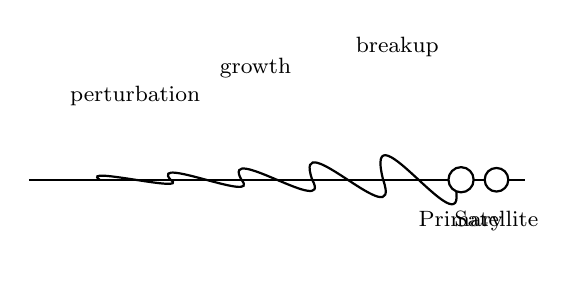
\begin{tikzpicture}[x=0.9cm,y=0.9cm]
  % Jet axis and growing disturbance
  \draw[line] (0,0) -- (7,0);
  \foreach \x/\a in {1/0.2,2/0.35,3/0.55,4/0.85,5/1.2}{
    \draw[line] (\x,0) .. controls +(-0.3,\a) and +(0.3,-\a) .. (\x+1,0);
  }

  % Annotations
  \node[note,above] at (1.5,0.9) {perturbation};
  \node[note,above] at (3.2,1.3) {growth};
  \node[note,above] at (5.2,1.6) {breakup};

  % Main drop and satellite (with labels placed below, slightly offset)
  \node[dot]                 (main) at (6.10,0) {};
  \node[dot,minimum size=3mm](sat)  at (6.60,0) {};

  \node[below=3pt of main, font=\footnotesize] {Primary};
  \node[below=3pt of sat,  font=\footnotesize] {Satellite};
\end{tikzpicture}
\end{document}
